\documentclass{article}
\usepackage[margin=1in]{geometry}
\usepackage[utf8]{inputenc}
\usepackage{amsmath}
\usepackage{amsfonts}
\usepackage{amssymb}
\usepackage{graphicx}

\title{Homework 2}
\author{Giacomo Cappelletto}
\date{\today}

\begin{document}

\maketitle

\section{Linear Transformations}

\subsection*{A)}
\subsubsection*{I)}
\[
	\begin{bmatrix}
		2 & 0 \\
		0 & 2
	\end{bmatrix}
\]
\subsubsection*{II)}

$$Scalar Matrix$$

\subsection*{B)}

\subsubsection*{I}

\[
	\begin{bmatrix}
		1 & -1 \\
		0 & 1
	\end{bmatrix}
\]
\subsubsection*{II)}

$$Horizontal shear$$

\subsection*{C)}

\subsubsection*{I)}

\[
	\begin{bmatrix}
		\cos(270^\circ) & -\sin(270^\circ) \\
		\sin(270^\circ) & \cos(270^\circ)
	\end{bmatrix}
	=
	\begin{bmatrix}
		0  & 1 \\
		-1 & 0
	\end{bmatrix}
\]

\subsubsection*{II)}

$$Rotation Matrix$$

\subsection{E)}

\subsubsection*{I)}

\[
	\begin{bmatrix}
		\cos(180^\circ) & -\sin(180^\circ) \\
		\sin(180^\circ) & \cos(180^\circ)
	\end{bmatrix}
	=
	\begin{bmatrix}
		1 & 0  \\
		0 & -1
	\end{bmatrix}
\]

\subsubsection*{II)}

$$Reflection Matrix$$

\subsection{F)}

\subsubsection*{I)}

\[
	\begin{bmatrix}
		1 & 0 \\
		0 & 0
	\end{bmatrix}
\]

\subsubsection*{II)}

$$Projection (matrix)$$

\section{Rotations}

\subsection*{A)}




$$	\cos(\theta + \phi) = \frac{v_1}{r} \Rightarrow v_1 = r \cdot \cos(\theta + \phi) $$
$$
	v= \begin{bmatrix}
		r \cdot \cos(\theta + \phi) \\
		r \cdot \sin(\theta + \phi)
	\end{bmatrix}
$$


$$	\cos(\theta) = \frac{z_1}{r} \Rightarrow z_1 = r \cdot \cos(\theta) $$
$$
	z= \begin{bmatrix}
		r \cdot \cos(\phi) \\
		r \cdot \sin(\phi)
	\end{bmatrix}
$$
\subsection*{B)}


Since
$$
	\cos(\theta + \phi) = \cos(\theta) \cos(\phi) - \sin(\theta) \sin(\phi)
$$
Then
$$
	v_1 = r \cdot \cos(\theta + \phi) = r \cdot \cos(\theta) \cos(\phi) - r \cdot \sin(\theta) \sin(\phi)
$$
\subsection*{C)}
Given
\[
	z_1 = r \cdot \cos(\theta) ,
	z_2 = \cdot \sin(\theta)
\]
Then
\[
	v_1 = z_1 \cdot \cos(\theta) - z_2 \cdot \sin(\theta)
\]

\subsection*{D)}

\[
	v_1 = \begin{bmatrix}
		\cos(\theta) & -\sin(\theta) \\
	\end{bmatrix}
	\cdot
	\begin{bmatrix}
		z_1 \\
		z_2
	\end{bmatrix}
	=
	z_1 \cdot \cos(\theta) - z_2 \cdot \sin(\theta)
\]

\subsection*{E)}
Since
$$
	\sin(\theta + \phi) = \sin(\theta) \cos(\phi) + \cos(\theta) \sin(\phi)
$$
Then
$$
	v_2 = r \cdot \sin(\theta + \phi) = r \cdot \sin(\theta) \cos(\phi) + r \cdot \cos(\theta) \sin(\phi)
$$

\subsection*{F)}
Given
\[
	z_1 = r \cdot \cos(\theta) ,
	z_2 = \cdot \sin(\theta)
\]
Then
\[
	v_2 = z_1 \cdot \sin(\theta) + z_2 \cdot \cos(\theta)
\]
\subsection*{G)}

\[
	v_2 = \begin{bmatrix}
		\sin(\theta) & \cos(\theta) \\
	\end{bmatrix}
	\cdot
	\begin{bmatrix}
		z_1 \\
		z_2
	\end{bmatrix}
	=
	z_1 \cdot \sin(\theta) + z_2 \cdot \cos(\theta)
\]

\subsection*{H)}

\[
	v = \begin{bmatrix}
		v_1 \\
		v_2
	\end{bmatrix}
	=
	\begin{bmatrix}
		\cos(\theta) & - \sin(\theta) \\
		\sin(\theta) & \cos(\theta)
	\end{bmatrix}
	\cdot
	\begin{bmatrix}
		z_1 \\
		z_2
	\end{bmatrix}
\]

\section{Homogeneous Transformations}

\subsection*{A)}
From the given T stops it is given that
$$L_1=1km, \space L_2=2km, \space L_3=3km$$
and
$$\theta_1=-45^\circ, \space \theta_2=45^\circ, \space \theta_3=45^\circ$$
Therefore the Homogeneous Transformation Matrices are
\[
	T_0= \begin{bmatrix}
		\cos(\theta_1) & -\sin(\theta_1) & 0 \\
		\sin(\theta_1) & \cos(\theta_1)  & 0 \\
		0              & 0               & 1
	\end{bmatrix}
	=
	\begin{bmatrix}
		\cos(-45^\circ) & -\sin(-45^\circ) & 0 \\
		\sin(-45^\circ) & \cos(-45^\circ)  & 0 \\
		0               & 0                & 1
	\end{bmatrix}
	=
	\begin{bmatrix}
		\frac{\sqrt{2}}{2}  & \frac{\sqrt{2}}{2} & 0 \\
		-\frac{\sqrt{2}}{2} & \frac{\sqrt{2}}{2} & 0 \\
		0                   & 0                  & 1
	\end{bmatrix}
\]
\[
	T_1= \begin{bmatrix}
		\cos(\theta_2) & -\sin(\theta_2) & L_1 \\
		\sin(\theta_2) & \cos(\theta_2)  & 0   \\
		0              & 0               & 1
	\end{bmatrix}
	=
	\begin{bmatrix}
		\cos(45^\circ) & -\sin(45^\circ) & 1 \\
		\sin(45^\circ) & \cos(45^\circ)  & 0 \\
		0              & 0               & 1
	\end{bmatrix}
	=
	\begin{bmatrix}
		\frac{\sqrt{2}}{2} & -\frac{\sqrt{2}}{2} & 1 \\
		\frac{\sqrt{2}}{2} & \frac{\sqrt{2}}{2}  & 0 \\
		0                  & 0                   & 1
	\end{bmatrix}
\]
\[
	T_2= \begin{bmatrix}
		\cos(\theta_3) & -\sin(\theta_3) & L_2 \\
		\sin(\theta_3) & \cos(\theta_3)  & 0   \\
		0              & 0               & 1
	\end{bmatrix}
	=
	\begin{bmatrix}
		\cos(45^\circ) & -\sin(45^\circ) & 2 \\
		\sin(45^\circ) & \cos(45^\circ)  & 0 \\
		0              & 0               & 1
	\end{bmatrix}
	=
	\begin{bmatrix}
		\frac{\sqrt{2}}{2} & -\frac{\sqrt{2}}{2} & 2 \\
		\frac{\sqrt{2}}{2} & \frac{\sqrt{2}}{2}  & 0 \\
		0                  & 0                   & 1
	\end{bmatrix}
\]

\[
	T_3= \begin{bmatrix}
		\cos(0) & -\sin(0) & L_3 \\
		\sin(0) & \cos(0)  & 0   \\
		0       & 0        & 1
	\end{bmatrix}
	=
	\begin{bmatrix}
		1 & 0 & 1 \\
		0 & 1 & 0 \\
		0 & 0 & 1
	\end{bmatrix}
\]

Working out $T_{ee}$ gives

\[
	T_{ee} = T_0 \cdot T_1 \cdot T_2 \cdot T_3
\]
\[
	=
	\begin{bmatrix}
		\frac{\sqrt{2}}{2}  & \frac{\sqrt{2}}{2} & 0 \\
		-\frac{\sqrt{2}}{2} & \frac{\sqrt{2}}{2} & 0 \\
		0                   & 0                  & 1
	\end{bmatrix}
	\times
	\begin{bmatrix}
		\frac{\sqrt{2}}{2} & -\frac{\sqrt{2}}{2} & 1 \\
		\frac{\sqrt{2}}{2} & \frac{\sqrt{2}}{2}  & 0 \\
		0                  & 0                   & 1
	\end{bmatrix}
	\times
	\begin{bmatrix}
		\frac{\sqrt{2}}{2} & -\frac{\sqrt{2}}{2} & 2 \\
		\frac{\sqrt{2}}{2} & \frac{\sqrt{2}}{2}  & 0 \\
		0                  & 0                   & 1
	\end{bmatrix}
	\times
	\begin{bmatrix}
		1 & 0 & 1 \\
		0 & 1 & 0 \\
		0 & 0 & 1
	\end{bmatrix}
\]
\[
	=
	\begin{bmatrix}
		1 & 0 & \frac{\sqrt{2}}{2}  \\
		0 & 1 & -\frac{\sqrt{2}}{2} \\
		0 & 0 & 1
	\end{bmatrix}
	\times
	\begin{bmatrix}
		\frac{\sqrt{2}}{2} & -\frac{\sqrt{2}}{2} & \frac{4+\sqrt{2}}{2} \\
		\frac{\sqrt{2}}{2} & \frac{\sqrt{2}}{2}  & \frac{\sqrt{2}}{2}   \\
		0                  & 0                   & 1
	\end{bmatrix}
\]
\[
	=
	\begin{bmatrix}
		\frac{\sqrt{2}}{2} & -\frac{\sqrt{2}}{2} & \frac{4+2\sqrt{2}}{2} \\
		\frac{\sqrt{2}}{2} & \frac{\sqrt{2}}{2}  & 0                     \\
		0                  & 0                   & 1
	\end{bmatrix}
\]
Therefore the position of Government center compared to BU central is
$$
	\begin{bmatrix}
		\frac{4+2\sqrt{2}}{2} \\
		0
	\end{bmatrix}
	=
	\begin{bmatrix}
		3.4142 \\
		0
	\end{bmatrix}
$$
and its orientation is
$$
	\begin{bmatrix}
		\frac{\sqrt{2}}{2} & -\frac{\sqrt{2}}{2} \\
		\frac{\sqrt{2}}{2} & \frac{\sqrt{2}}{2}
	\end{bmatrix}
	\space
	(\theta = 45^\circ)
$$

\section{MATLAB}

\sloppy
\setlength{\parindent}{0pt}

\begin{verbatim}
% Put together a list of `n` 2x2 simple geometric transformations
clear
A_lst(:,:,1) = [1 0; 0 1];                           % First matrix
A_lst(:,:,2) = [-1 0; 0 1];                          % Second matrix
A_lst(:,:,3) = [1 0; 0 -1];                          % Third matrix
A_lst(:,:,4) = [cos(pi/2) -sin(pi/2); sin(pi/2) cos(pi/2)]; % Fourth matrix
A_lst(:,:,5) = [1/2 0; 0 1];                         % Fifth matrix
A_lst(:,:,6) = [1 0; 0 1/2];                         % Sixth matrix
A_lst(:,:,7) = [1 0.5; 0 1];                           % Seventh matrix
A_lst(:,:,8) = [1 0; 0.5 1];                           % Eighth matrix

% Define the house
H = [[0;0], [0;1], [1;1.5], [1;1], [1;0], [0;0]];

% Create the first figure
figure(1)

% Plot the house
plot(H(1,:), H(2,:), '-o', 'Color', 'blue', 'MarkerFaceColor', 'red')
title('Original image')

xlim([-2 2])
axis equal

% Get the number of 2x2 matrices
numMatrices = size(A_lst,3);

% Create a second figure
figure(2)
set(gcf, 'Position', [100, 100, 800, 1200]);

transf = {"Scaling by factor of 1", "Reflection about y-axis", "Reflection about x-axis", "Rotation by 90°", "Horizontal Shrink by factor of 1/2", "Vertical shrink by factor of 1/2", "Horizontal shear by 1/2", "Vertical Shear by 1/2"};

for i = 1:numMatrices
    H_transformed = A_lst(:,:,i) * H;
    subplot(ceil(sqrt(numMatrices)), ceil(sqrt(numMatrices)), i); % Create subplots
    plot(H_transformed(1,:), H_transformed(2,:), '-o', 'Color', 'blue', 'MarkerFaceColor', 'red');
    title(['Transformation ' transf(i)], "FontSize", 10);
    xlim([-2 2]);
    ylim([-2 2]);
    axis equal;
end
\end{verbatim}

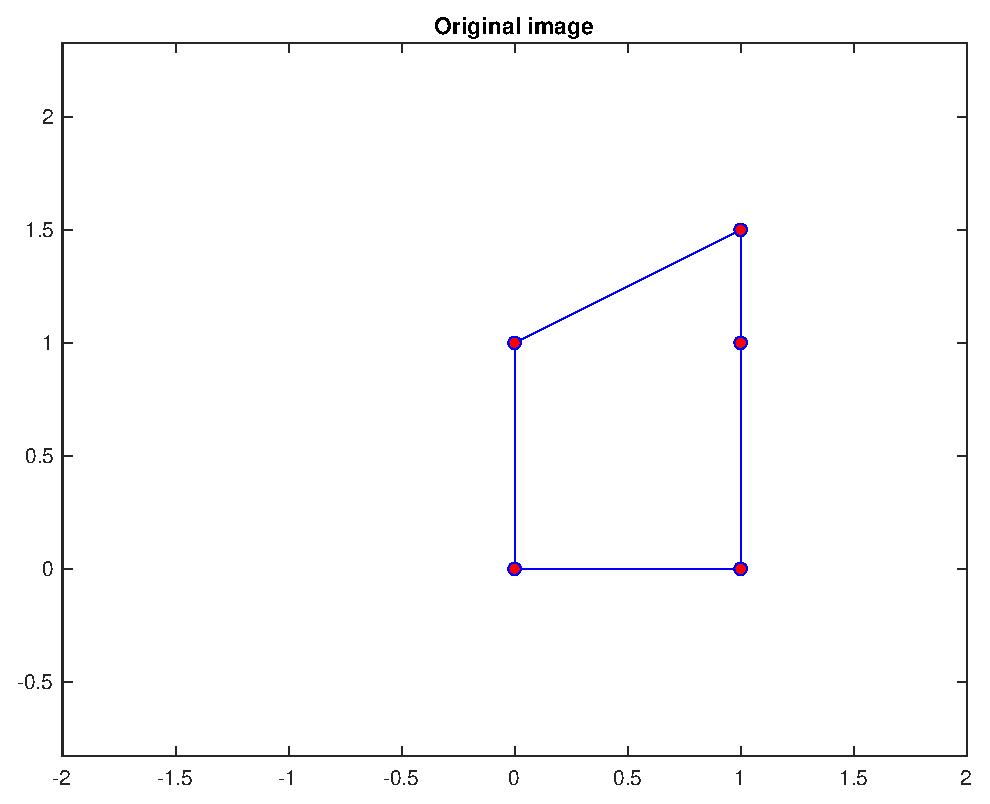
\includegraphics [width=2in]{transformations_01.eps}
\vspace{1cm}
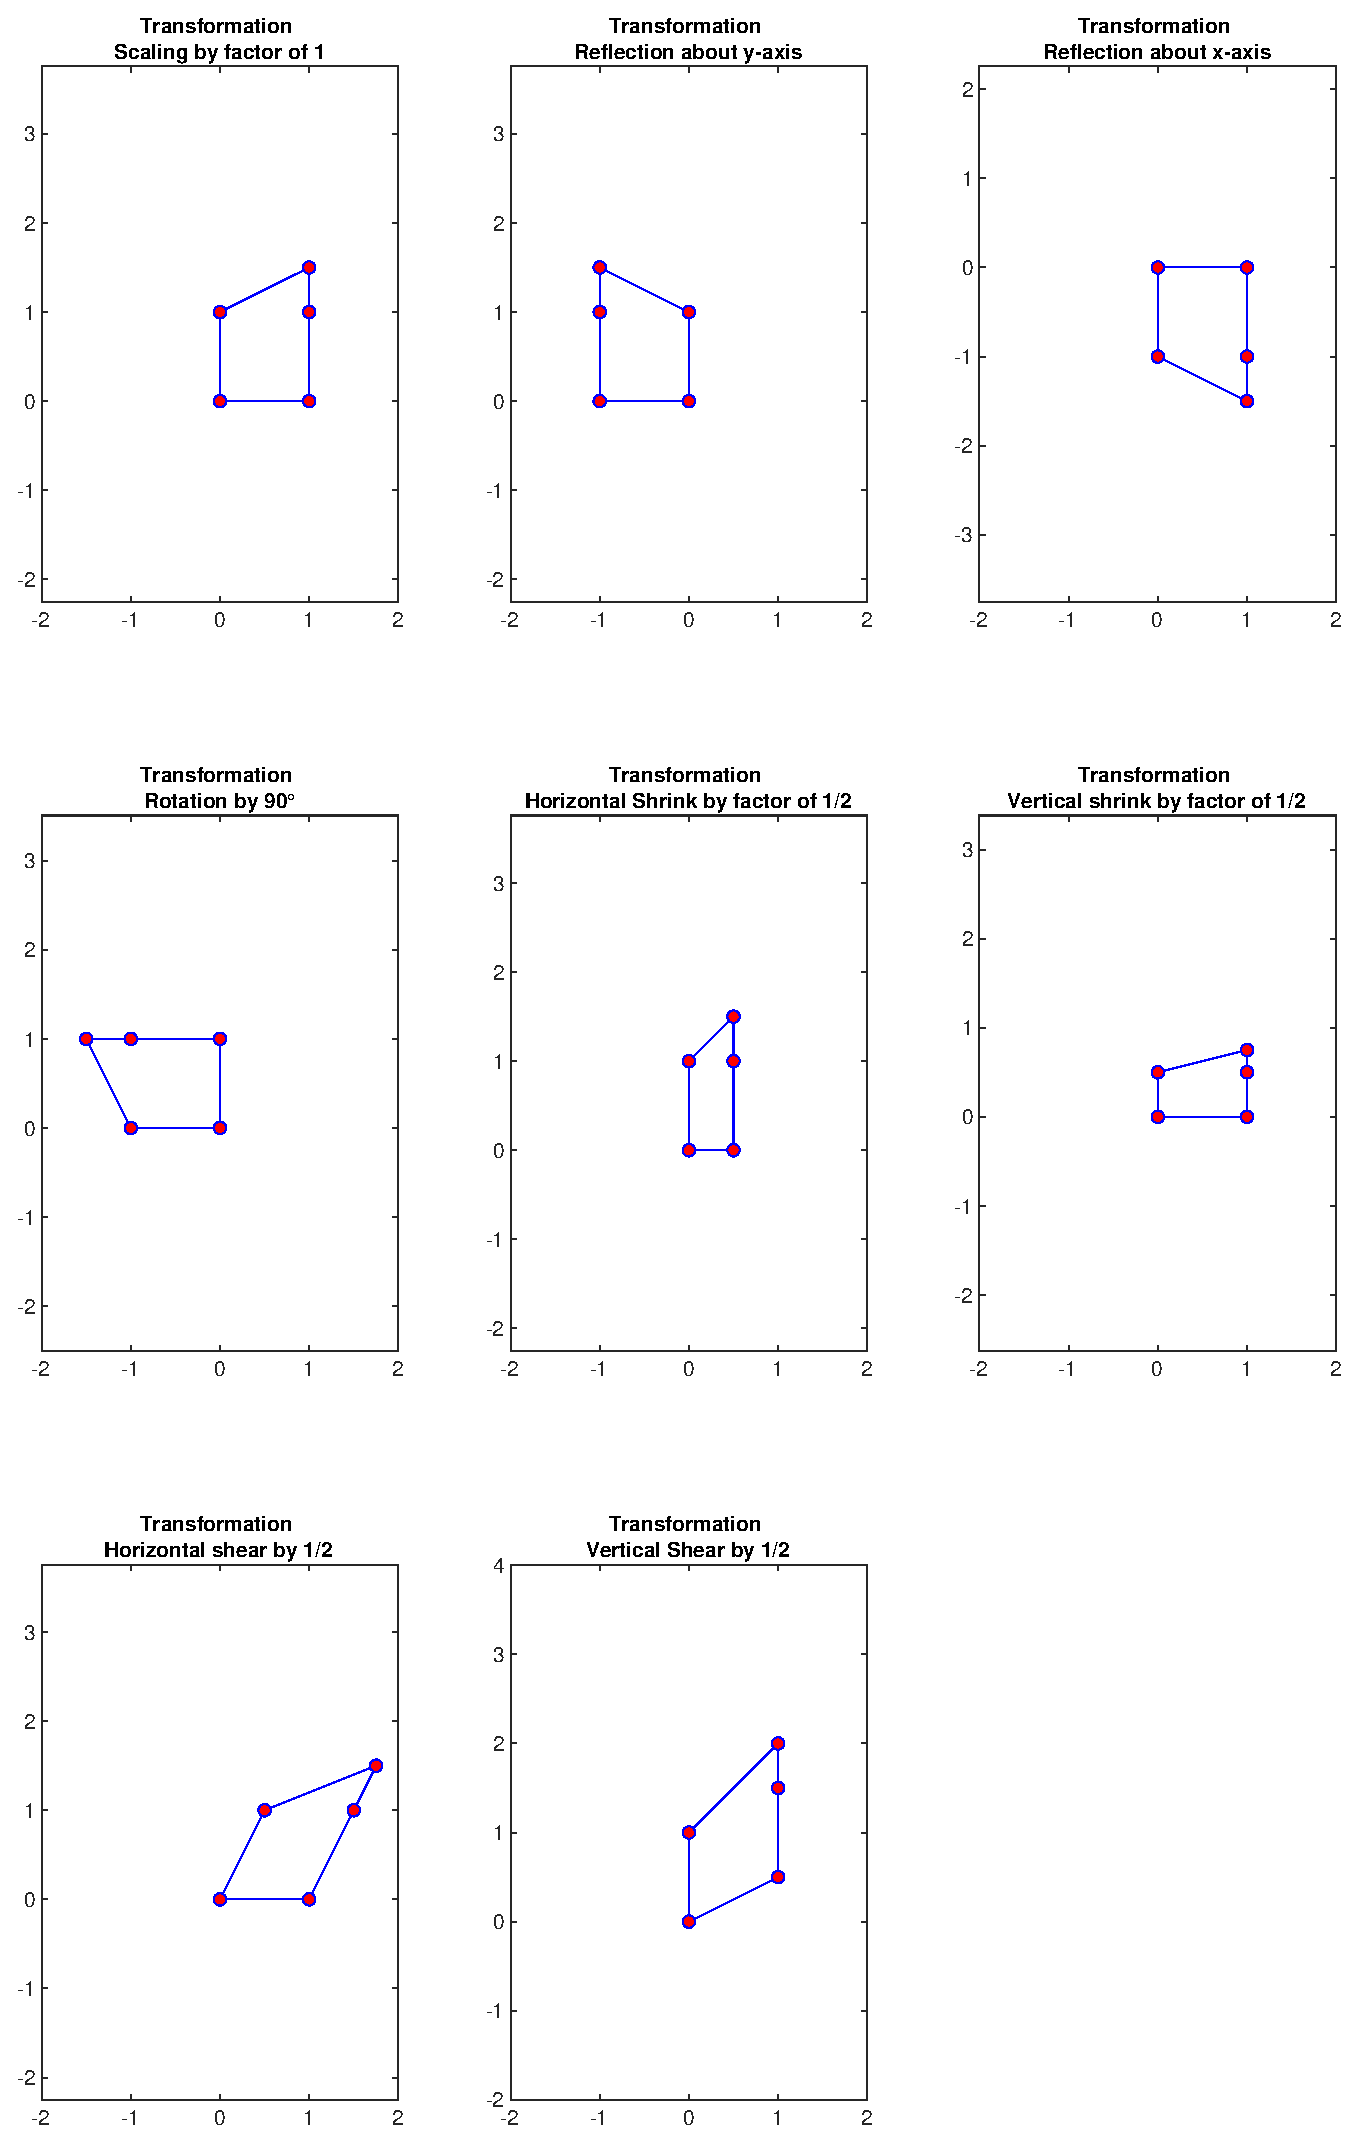
\includegraphics [width=5in]{transformations_02.eps}


\end{document}